\section{Objectives}
\label{sec:objectives}
The life-cycle of a Cloud-based IoT application is composed by several stages,
as illustrated in the Figure \ref{fig:life-cycle}. Some of the stages are placed in
the smart place while others are placed in the Cloud.
% Application Life-cycle
\begin{figure}[h!]
  \centering
  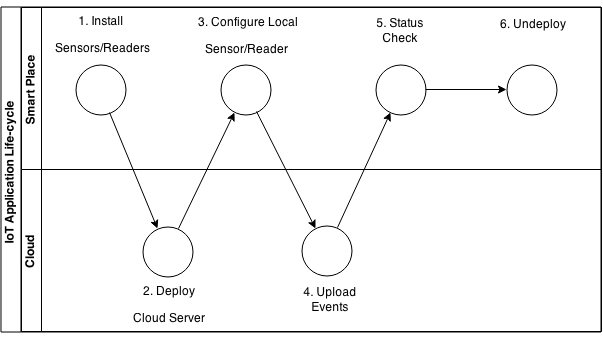
\includegraphics[width=\textwidth]{./images/life-cycle}
  \caption{IoT application life-cycle.}
  \label{fig:life-cycle}
\end{figure}

The life-cycle of an IoT application starts with the installation of the sensors and
readers in the smart place (step 1). The next step consists in preparation to
process the events sent by the smart objects. First the application must be deployed at
the Cloud in order to be able to receive the events (step 2). After that the installed
sensors and readers must be configured to send the generated events to the application that is
running in the Cloud (step 3). At this point the smart place is already configured to
support the processing of events generated by smart objects (step 4).\\

- Falar do objectivo principal : automated deployment\\
- Falar do objectivo secundario : application monitoring\\

A very important point is to assure that the smart place is working according with the
desired Quality of Service (QoS). QoS is a concept that encompasses a number of nonfunctional
properties such as availability, reliability, price and reputation \cite{o2002s}.
Thus in order to monitoring the performance of the application in the smart place (step 5),
these properties must be agreed between the customer and the Cloud provider.
This agreement between the customer and the service provider is know as Service Level Agreement (SLA).
The SLA defines the terms and conditions of service quality that a service provider delivers
to service requesters based on the desired \textit{QoS} \cite{zeng2004qos}. The final stage
that an IoT application can reach is its undeployment, which means that the smart place is deactivated (step 6).\\

The objective of this work is to decrease the complexity of deployment and management
of Cloud-based IoT applications in a smart place. Usually the deployment of such applications
is performed by a technician that manually configures and installs the components of the application.
In order to reduce the complexity of this process, deployment process of the application will be automated.
That is achieved by performing the deployment through Cloud Orchestration tools, that allows the specification
of the components and the relations between them in a high-level perspective and also provisioning
the necessary resources at the Cloud in a effective way. These tools also allows the monitoring
of applications during its life-cycle. However, these tools do not solve all problems.
In particular, IoT applications require a software stack that usually is composed by a database,
a web server and the event processing software. But orchestration tools normally lack the
integration of the event processing software with the other components. Thus, to support the
integration of such components these tools must be extend to support the event processing software.\\

Managing IoT applications through an Orchestrator tool requires an elevated technical knowledge.
To allow that non-technical users can perform the managing operations having in perspective
the high-level business rules of the smart place, the main objective of this work is to permit
that non-technical users can perform the management of smart places only having in mind the business
rules of that particular place. To achieve that, these high-level rules must be translated to a more
low-level rules that can be expressed in terms of non-functional requirements, SLAs, that can be
used to estimate the resources needed by the application in order to have an acceptable \textit{QoS}.
In the other hand, to allow those non-technical users to monitor the smart place, these SLAs must
be translated to high-level rules that can be expressed in terms of business rules of a given smart place.
For instance, if a smart place has a flow of people of 500 persons per day, that business rule will be
translated to a SLA that express the amount of storage and bandwidth required to ensure the \textit{QoS}
of the application. Furthermore, by monitoring the service level offered by the Cloud providers it will be
possible to determine if the Cloud is overloaded with the amount of data generated by the smart place or not.
